% Chapter Three: the salt roads, their brokers, and the effect of the plague years.
\chapter{The Salt Roads}
\label{ch:salt}

\section{The Shape of the Network}

Figure~\ref{fig:network} shows the overland network reconstructed from the registers for the decade 1400--1409. Line weight is proportional to the estimated weight of goods carried. Two features stand out. The first is the dominance of the Lüneburg--Lübeck axis, which carried nearly half of all recorded salt. The second is the position of Mölln, through which every route from the salt works to the eastern Baltic ports had to pass.

\begin{figure}[tbp]
  \centering
  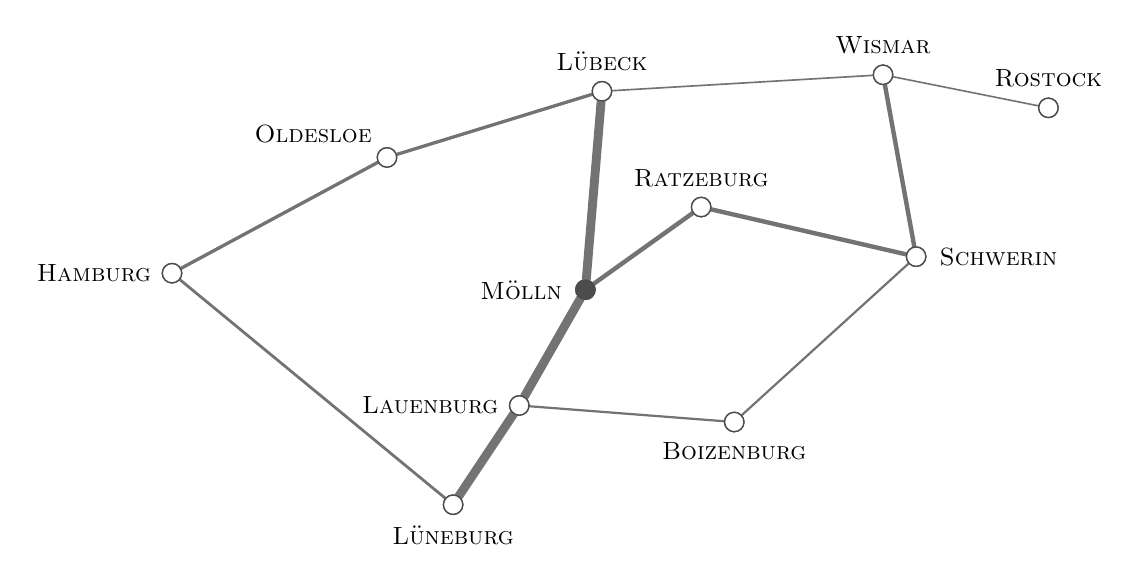
\begin{tikzpicture}[x=1.05cm,y=1.05cm,
      town/.style={circle, draw=black!70, fill=white, line width=0.5pt,
        minimum size=7pt, inner sep=0pt},
      broker/.style={town, fill=black!70},
      lbl/.style={font=\small\scshape},
      route/.style={draw=black!55, line cap=round}]
    \node[town]   (hh)  at (0,2.2)   {};
    \node[town]   (lue) at (5.2,4.4) {};
    \node[town]   (wis) at (8.6,4.6) {};
    \node[town]   (ros) at (10.6,4.2){};
    \node[broker] (mol) at (5.0,2.0) {};
    \node[town]   (old) at (2.6,3.6) {};
    \node[town]   (rat) at (6.4,3.0) {};
    \node[town]   (lau) at (4.2,0.6) {};
    \node[town]   (lun) at (3.4,-0.6){};
    \node[town]   (boi) at (6.8,0.4) {};
    \node[town]   (sch) at (9.0,2.4) {};
    \draw[route, line width=3.2pt] (lun) -- (lau) -- (mol) -- (lue);
    \draw[route, line width=1.6pt] (mol) -- (rat) -- (sch) -- (wis);
    \draw[route, line width=1.2pt] (hh) -- (old) -- (lue);
    \draw[route, line width=1.0pt] (lun) -- (hh);
    \draw[route, line width=0.8pt] (lau) -- (boi) -- (sch);
    \draw[route, line width=0.6pt] (wis) -- (ros);
    \draw[route, line width=0.6pt] (lue) -- (wis);
    \foreach \n in {hh,lue,wis,ros,old,rat,lau,lun,boi,sch} {\node[town] at (\n) {};}
    \node[broker] at (mol) {};
    \node[lbl, left=4pt]  at (hh)  {Hamburg};
    \node[lbl, above=4pt] at (lue) {Lübeck};
    \node[lbl, above=4pt] at (wis) {Wismar};
    \node[lbl, above=4pt] at (ros) {Rostock};
    \node[lbl, left=5pt]  at (mol) {Mölln};
    \node[lbl, above left=2pt] at (old) {Oldesloe};
    \node[lbl, above=4pt] at (rat) {Ratzeburg};
    \node[lbl, left=4pt]  at (lau) {Lauenburg};
    \node[lbl, below=4pt] at (lun) {Lüneburg};
    \node[lbl, below=4pt] at (boi) {Boizenburg};
    \node[lbl, right=5pt] at (sch) {Schwerin};
  \end{tikzpicture}
  \caption[Overland routes of the southern Baltic, 1400--1409]{Overland routes of the southern Baltic, 1400--1409. Line weight is proportional to recorded tonnage; the filled node marks the principal broker.}
  \label{fig:network}
\end{figure}

The network is sparse. Of the 55 possible connections between its eleven principal towns, only twelve carry recorded traffic. Yet the mean shortest path between any two towns is just 2.4 steps, the hallmark of a network that is cheap to maintain and still well integrated.\footnote{By comparison, a random network with the same number of towns and connections would have a mean path length of about 2.9 steps.}

\section{Distance, Tolls and Trade}

Estimating Equation~\eqref{eq:loggravity} on the full set of town pairs yields a distance elasticity of $\hat{\gamma} = 1.31$ and a toll coefficient of $\hat{\delta} = 0.22$. Each additional toll station thus reduced expected trade by roughly a fifth, holding distance constant. Table~\ref{tab:gravity} reports the estimates for the two halves of the period.

\begin{table}[tbp]
  \centering
  \caption{Gravity model estimates before and after 1400}
  \label{tab:gravity}
  \begin{tabular}{@{}l r r r@{}}
    \toprule
    & 1350--1399 & 1400--1450 & All years \\
    \midrule
    Origin size, $\alpha$      & 0.84 & 0.91 & 0.87 \\
    Destination size, $\beta$  & 0.72 & 0.79 & 0.76 \\
    Distance, $\gamma$         & 1.44 & 1.18 & 1.31 \\
    Tolls, $\delta$            & 0.17 & 0.27 & 0.22 \\
    \midrule
    Town pairs                 & 231  & 274  & 412  \\
    $R^2$                      & 0.58 & 0.63 & 0.61 \\
    \bottomrule
  \end{tabular}
\end{table}

The contrast between the two halves is the most important result of this chapter. After 1400, distance mattered less and tolls mattered more. Roads had improved, carts had grown larger, and the cost of moving a barrel one more mile had fallen. But the toll stations had multiplied and their rates had risen, so that the decisive cost of trade was increasingly a political one \parencite{brandt1997}.

\section{The Brokers}

Betweenness centrality, computed with Equation~\eqref{eq:betweenness}, confirms what the map suggests. Mölln's score is more than twice that of any other town, and Lauenburg and Ratzeburg follow at a distance. None of these was a large place; Mölln had perhaps 1,500 inhabitants. Their importance lay entirely in their position.

Lübeck understood this. In 1359 the city acquired Mölln and its toll from the dukes of Saxe-Lauenburg by way of a mortgage that it never allowed to be redeemed \parencite{hammel1988}. The purchase has usually been explained as a matter of security. The network evidence suggests a simpler motive: by owning the broker, Lübeck owned the route.

\subsection{Reorganisation after the Plague}

The plague of 1349--1351 and its recurrence in 1374 reduced the population of the region by perhaps a third. One might expect the network to have contracted in proportion. It did not. The number of active routes fell by only two, and the share of traffic passing through the three principal brokers rose from 54 to 68 per cent. Fewer carriers travelled on fewer roads, and those roads were the ones that the brokers controlled.

\section{Silver and the Return Trade}

Salt travelled north; silver travelled south. The registers record the return cargoes far less carefully, because coin and bullion in the hands of merchants were often exempt from toll, but the merchant letters fill much of the gap. Partners of the Castorp firm wrote of settling salt purchases at Lüneburg with Saxon silver brought up from the Erzgebirge by way of Magdeburg, and of carrying the surplus to Lübeck for shipment to Bergen and Novgorod \parencite{selzer2003}.

The return trade matters for the argument because it explains why the brokers could raise their tolls without driving traffic away. A carter who brought salt to Lübeck could expect a paying cargo for the journey home, so that the cost of a toll was spread across two loads rather than one. The gravity estimates in Table~\ref{tab:gravity}, which treat each direction separately, therefore overstate the burden that tolls placed on any single round trip, though not the political leverage that they gave to those who collected them.\footnote{A model that pairs outbound and return flows would require matching individual carters across registers, which is possible for only 212 of the 4,118 entries.}

\section{Conclusion}

The overland network of the southern Baltic was neither a minor appendage to the maritime trade nor a simple reflection of it. Its structure created positions of power that had little to do with size or wealth, and the cities that grasped this, above all Lübeck, turned that structure to their advantage. When, in the fifteenth century, territorial princes began to reclaim the inland toll stations, they struck at the foundation on which Hanseatic commerce had quietly rested.
